\section{Analyse des données}

\subsection{Données physiques}

\subsubsection*{Heure des données}

Pour un dataframe données, l'heure de chaque ligne est toujours comprise dans une plage de temps très restreinte (aux alentour de 1h maximum d'écart). Par exemple, pour le dataframe 1, l'heure des données est comprise entre 18h23 et 19h03.

De plus, les dataframes 1 et 3 ont des données prises le même jour.

\subsubsection*{Colonnes Tank}

\begin{figure}[H]
  \centering
  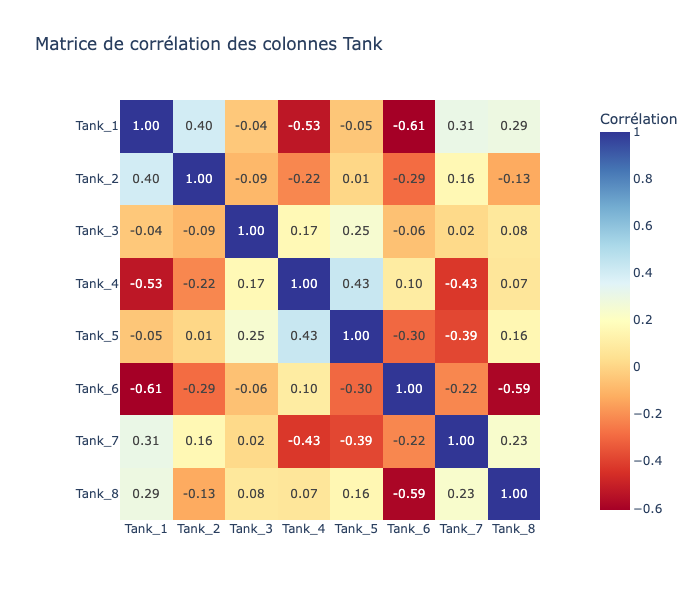
\includegraphics[width=0.6\textwidth]{figures/physical-analysis/tank-correlation.png}
  \caption{Matrice de corrélation des colonnes tanks}
  \label{fig:tank-correlation}
\end{figure}

Comme le montre la figure \ref{fig:tank-correlation}, il n'y a pas de tendance globale entre les colonnes \texttt{Tank} des différents fichiers. Il y aurait peut-être un lien entre les tanks proches, mais cela reste à confirmer.

\subsubsection*{Colonnes Pump}

\begin{figure}[H]
  \centering
  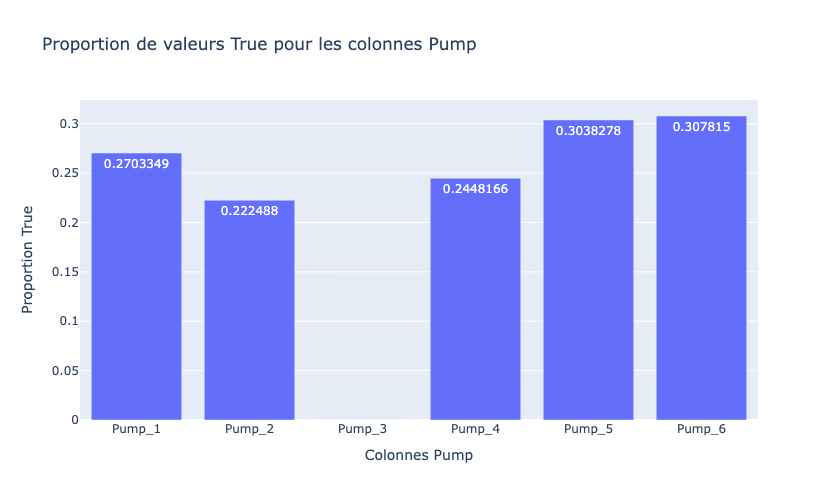
\includegraphics[width=0.6\textwidth]{figures/physical-analysis/pump_proportion.png}
  \caption{Proportion des valeurs de la colonne Pump}
  \label{fig:pump-proportion}
\end{figure}

La figure \ref{fig:pump-proportion} montre que les colonnes \texttt{pump} sont majoritairement à \texttt{false}. De plus, la colonne \texttt{Pump\_3} est toujours à \texttt{false} et ce quel que soit le dataframe.

\subsubsection*{Colonnes Flow\_sensor}

\begin{figure}[H]
  \centering
  % Première ligne
  \begin{minipage}[b]{0.45\textwidth}
    \centering
    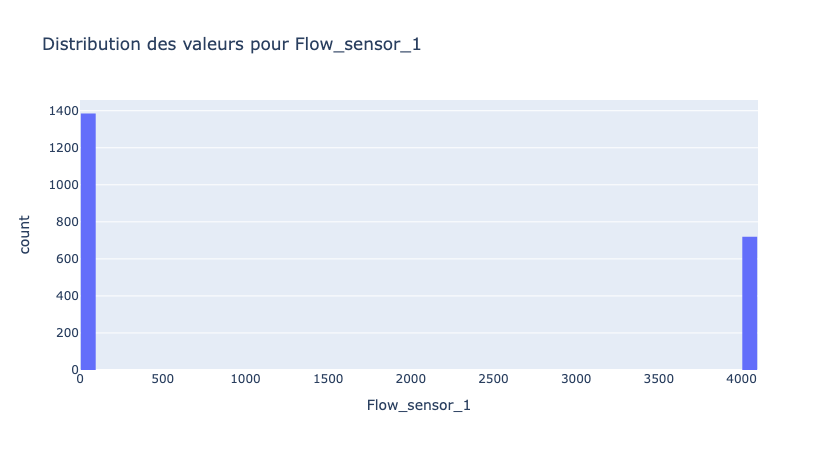
\includegraphics[width=\textwidth]{figures/physical-analysis/flowsensor1.png}
  \end{minipage}
  \hfill
  \begin{minipage}[b]{0.45\textwidth}
    \centering
    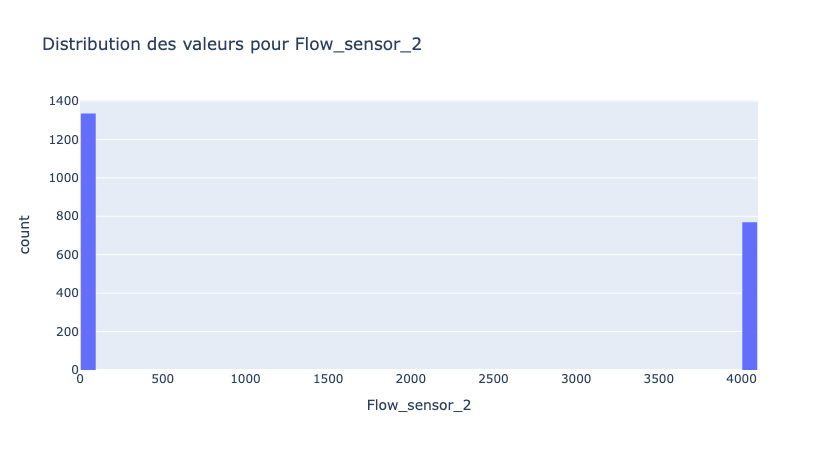
\includegraphics[width=\textwidth]{figures/physical-analysis/flowsensor2.png}
  \end{minipage}
  \vspace{1em} % Espace vertical entre les lignes
  % Deuxième ligne
  \begin{minipage}[b]{0.45\textwidth}
    \centering
    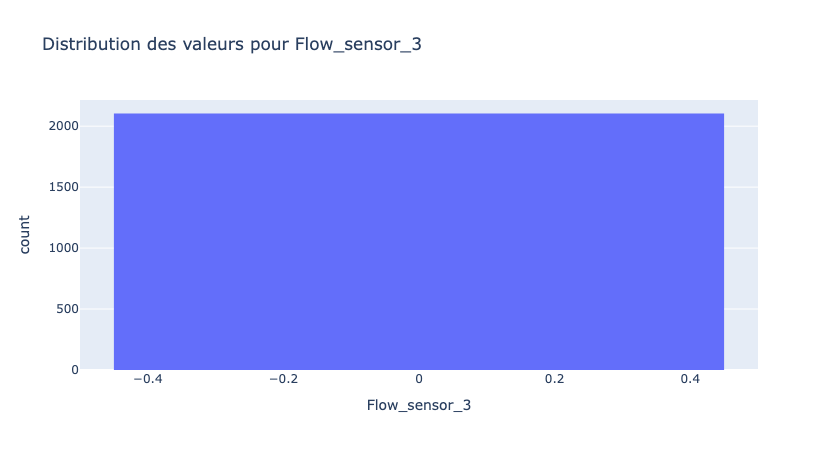
\includegraphics[width=\textwidth]{figures/physical-analysis/flowsensor3.png}
  \end{minipage}
  \hfill
  \begin{minipage}[b]{0.45\textwidth}
    \centering
    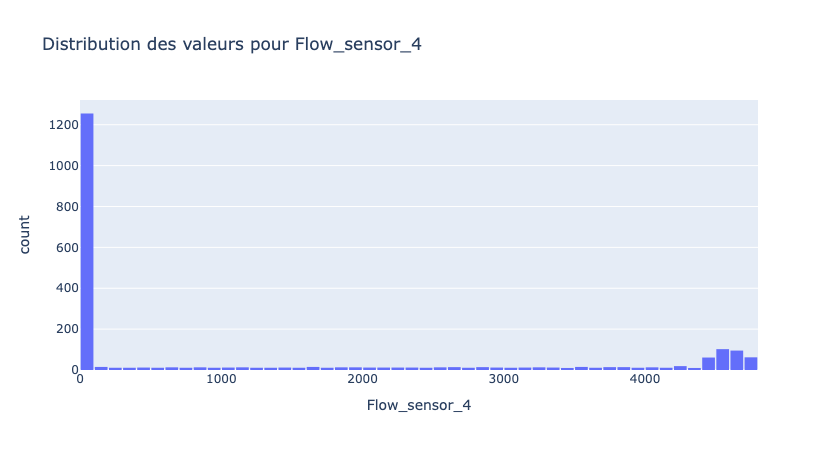
\includegraphics[width=\textwidth]{figures/physical-analysis/flowsensor4.png}
  \end{minipage}
  \caption{Distribution des valeurs de \texttt{flow\_sensor}}
  \label{fig:flowsensor}
\end{figure}
La figure \ref{fig:flowsensor} montre la distribution des valeurs de la colonne \texttt{flow\_sensor}. On peut en tirer les conclusions suivantes :
\begin{itemize}
  \item Pour les capteurs \texttt{flow\_sensor\_1} et \texttt{flow\_sensor\_2}, les valeurs sont uniquement 0, 100 et 4000.
  \item Le capteur \texttt{flow\_sensor\_3} ne présente que des valeurs à 0.
  \item Les valeurs du capteur \texttt{flow\_sensor\_4} sont réparties entre 0 et 5000. Cette répartition n'est pas uniforme mais il y a des valeurs quasiment pour chaque intervalle.
  \item Quel que soit le sensor, il y a toujours une majorité de valeurs à 0.
\end{itemize}

Cette figure ne montre les résultats que pour 1 dataframes mais la tendance globale est la même pour les autres.

\subsubsection*{Colonnes Valv}

\begin{figure}[H]
  \centering
  % Première ligne
  \begin{minipage}[b]{0.45\textwidth}
    \centering
    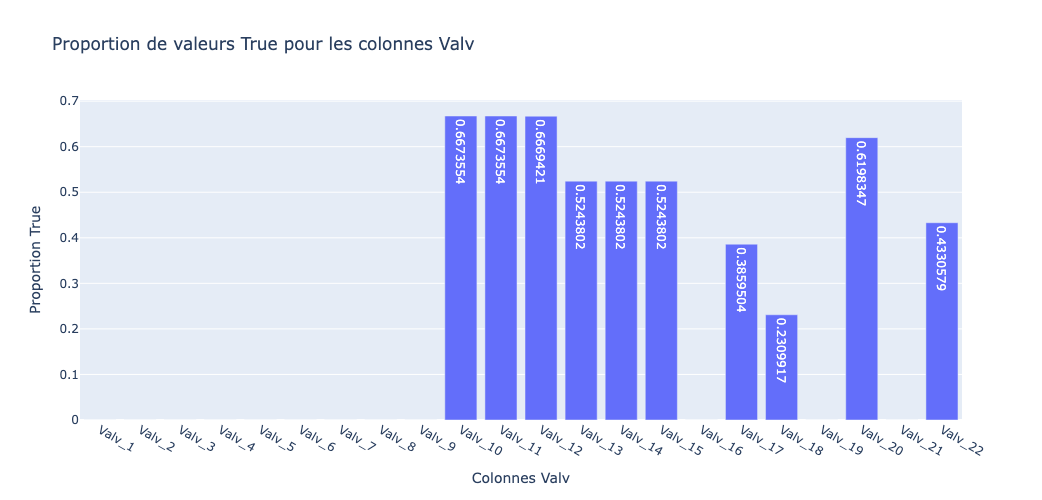
\includegraphics[width=\textwidth]{figures/physical-analysis/df1valve.png}
  \end{minipage}
  \hfill
  \begin{minipage}[b]{0.45\textwidth}
    \centering
    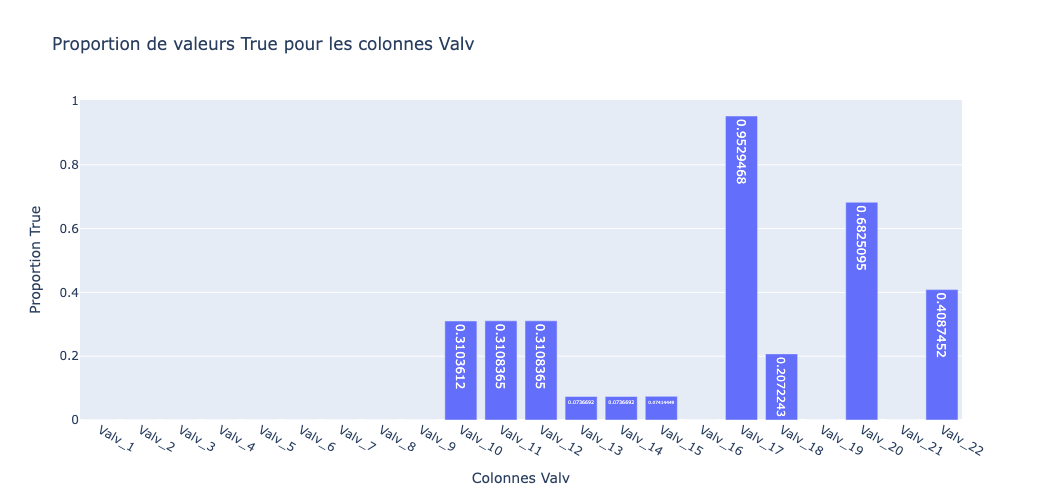
\includegraphics[width=\textwidth]{figures/physical-analysis/df2valve.png}
  \end{minipage}
  \vspace{1em} % Espace vertical entre les lignes
  % Deuxième ligne
  \begin{minipage}[b]{0.45\textwidth}
    \centering
    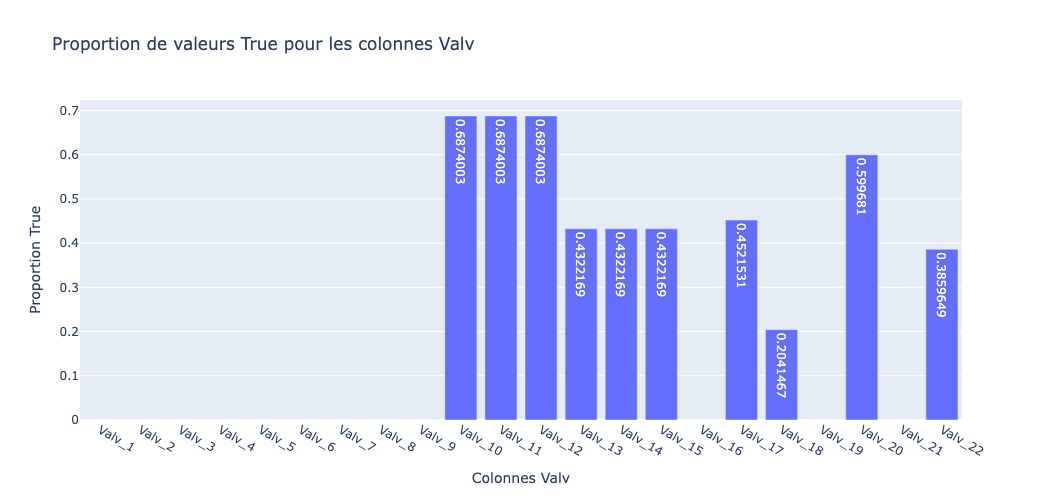
\includegraphics[width=\textwidth]{figures/physical-analysis/df3valve.png}
  \end{minipage}
  \hfill
  \begin{minipage}[b]{0.45\textwidth}
    \centering
    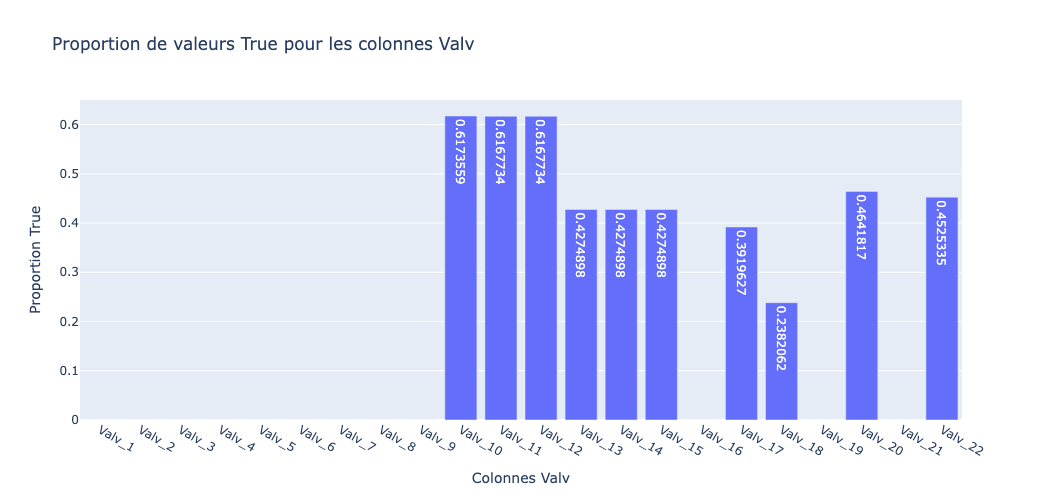
\includegraphics[width=\textwidth]{figures/physical-analysis/df4valve.png}
  \end{minipage}
  \caption{Distribution des valeurs pour les colonnes \texttt{valv} pour chaque dataframe}
  \label{fig:valv}
\end{figure}

Concernant les colonnes \texttt{valv}, la figure \ref{fig:valv} montre que la proportion de true est souvent similaire pour une valve données. Cela semble s'appliquer sur tous les dataframes sauf pour le dataframe 2 où la proportion de \texttt{true} est différente.

Par ailleurs, les 9 première valves sont toujours à \texttt{false} et il est donc possible de les ignorer.

\subsubsection*{Distribution des labels}

\begin{figure}[H]
  \centering
  % Première ligne
  \begin{minipage}[b]{0.45\textwidth}
    \centering
    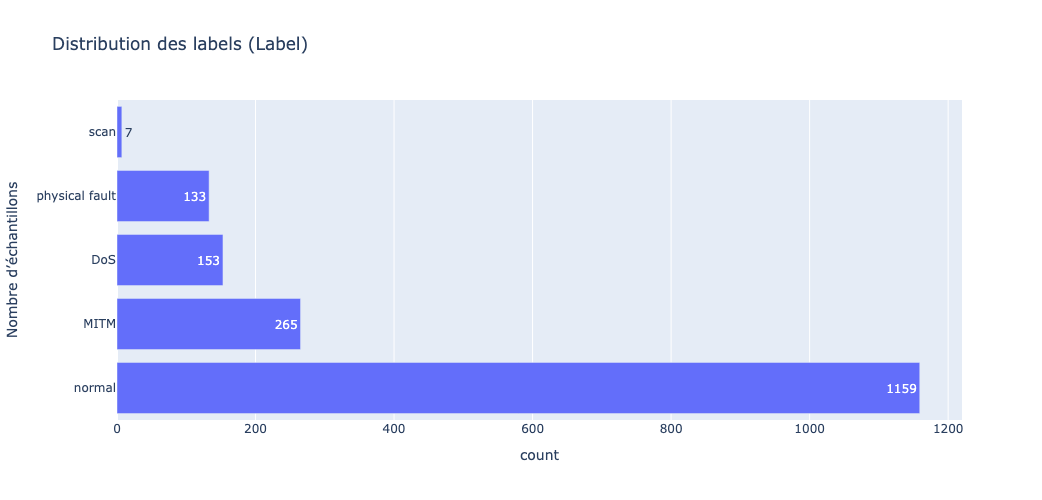
\includegraphics[width=\textwidth]{figures/physical-analysis/distriblabel.png}
  \end{minipage}
  \hfill
  \begin{minipage}[b]{0.45\textwidth}
    \centering
    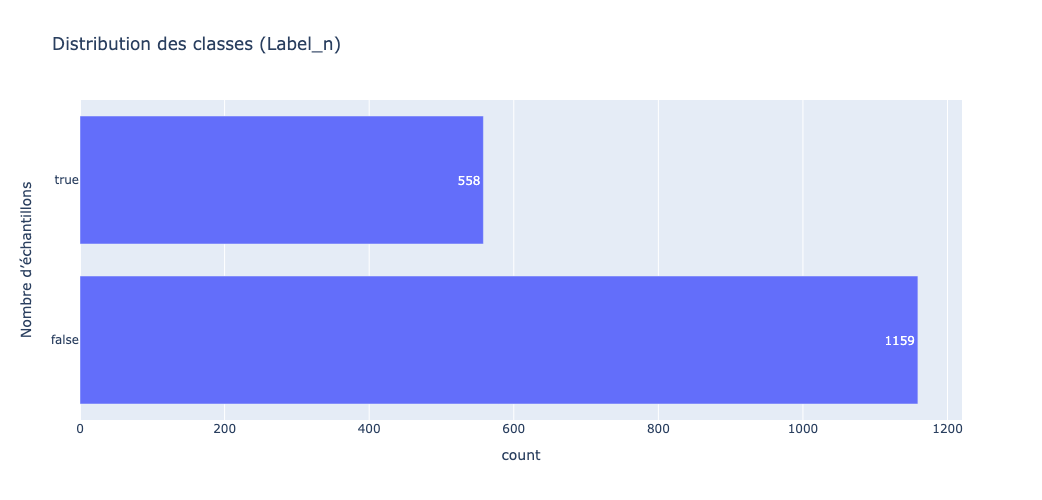
\includegraphics[width=\textwidth]{figures/physical-analysis/distriblabel_n.png}
  \end{minipage}
  \caption{Distribution de \texttt{label} et \texttt{label\_n}}
  \label{fig:labels}
\end{figure}

La figure \ref{fig:labels} montre qu'il y a une majorité de valeurs \texttt{normal} pour la colonne \texttt{label}, qui suit le nombre de valeurs \texttt{false} de la colonne \texttt{label\_n}.

Ces deux données sont donc liées et il est possible de ne pas utiliser la colonne \texttt{label\_n}.

\subsubsection*{Distribution des valeurs de tank}

\begin{figure}[H]
  \centering
  % Première ligne
  \begin{minipage}[b]{0.45\textwidth}
    \centering
    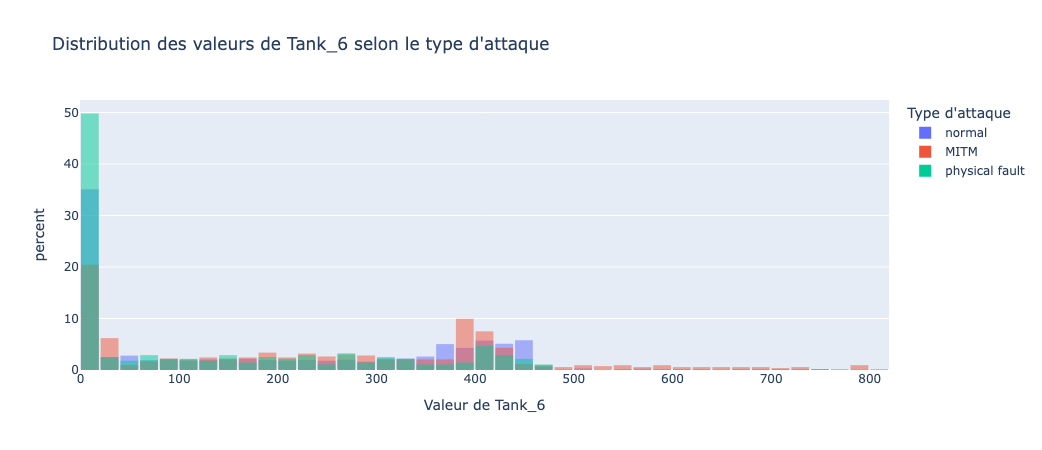
\includegraphics[width=\textwidth]{figures/physical-analysis/newplot1.png}
  \end{minipage}
  \hfill
  \begin{minipage}[b]{0.45\textwidth}
    \centering
    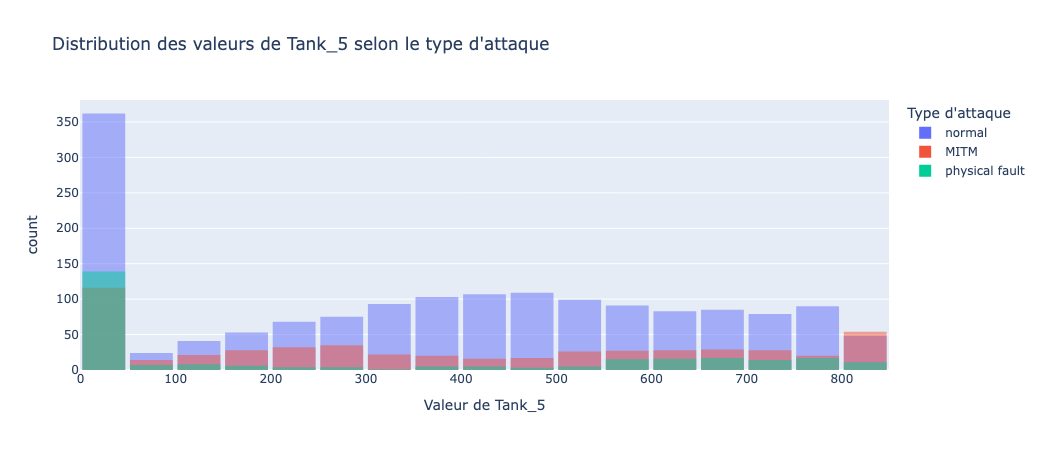
\includegraphics[width=\textwidth]{figures/physical-analysis/newplot2.png}
  \end{minipage}
  \caption{Distribution des valeurs de \texttt{tank} selon le type d'attaque}
  \label{fig:tank}
\end{figure}

Un graphe a été généré pour chaque dataframe et pour chaque tank mais il n'y a pas de tendance claire. Il est donc difficile de tirer des conclusions sur la distribution des valeurs de tank.

\subsubsection*{Distriubution selon le nombre de valves}

\begin{figure}[H]
  \centering
  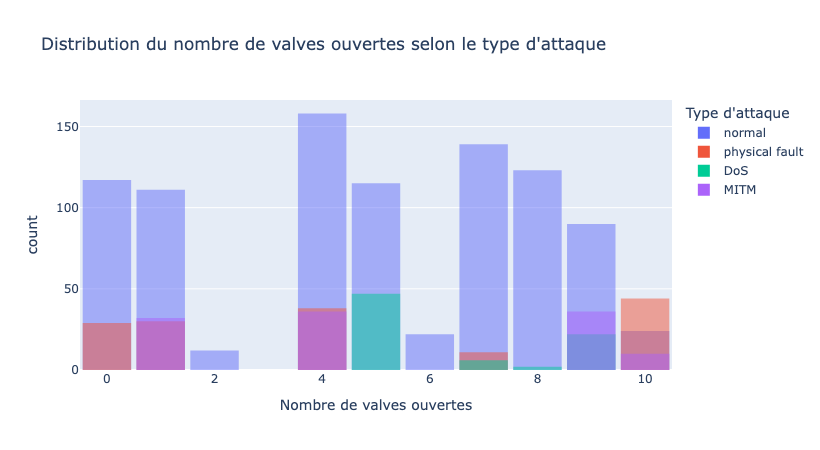
\includegraphics[width=0.6\textwidth]{figures/physical-analysis/newplot.png}
  \caption{Distribution du nombre d'attaques en fonction du nombre de valves ouvertes}
  \label{fig:valv-distribution}
\end{figure}

Cette figure montre qu'il n'y a pas de tendance claire entre le nombre d'attaques et le nombre de valves ouvertes.

\subsubsection*{Distribution des valeurs de \texttt{pump}}

\begin{figure}[H]
  \centering
  % Première ligne
  \begin{minipage}[b]{0.45\textwidth}
    \centering
    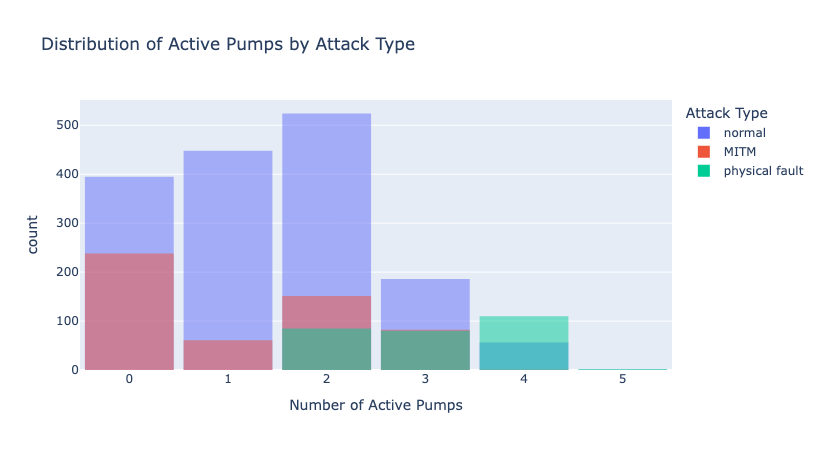
\includegraphics[width=\textwidth]{figures/physical-analysis/pump1.png}
  \end{minipage}
  \hfill
  \begin{minipage}[b]{0.45\textwidth}
    \centering
    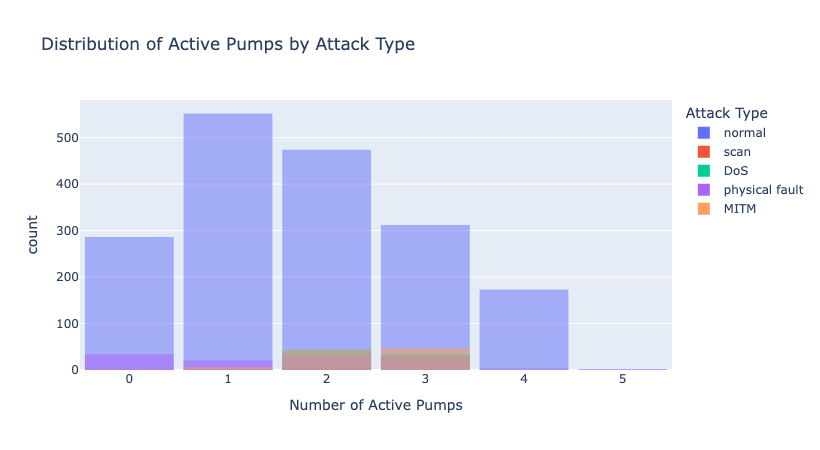
\includegraphics[width=\textwidth]{figures/physical-analysis/pump2.png}
  \end{minipage}
  \vspace{1em} % Espace vertical entre les lignes
  % Deuxième ligne
  \begin{minipage}[b]{0.45\textwidth}
    \centering
    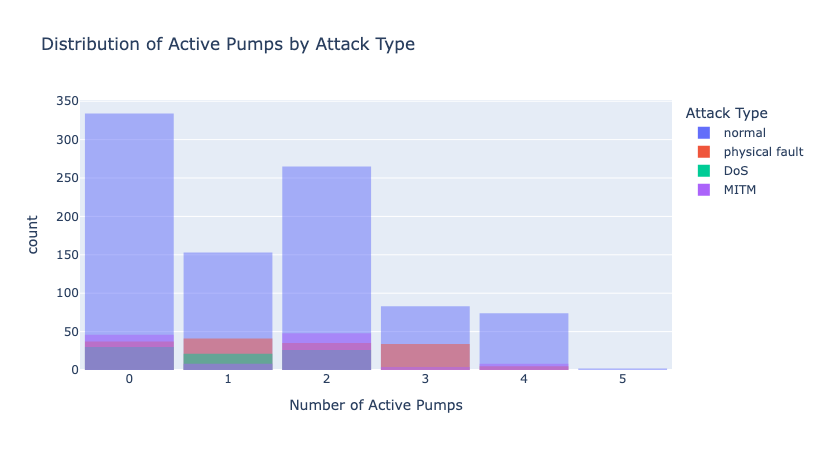
\includegraphics[width=\textwidth]{figures/physical-analysis/pump3.png}
  \end{minipage}
  \hfill
  \begin{minipage}[b]{0.45\textwidth}
    \centering
    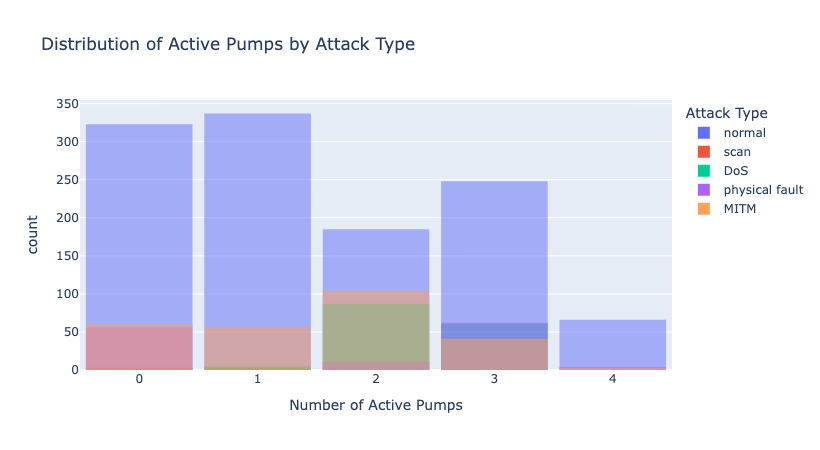
\includegraphics[width=\textwidth]{figures/physical-analysis/pump4.png}
  \end{minipage}
  \caption{Distribution du nombre d'attaques en fonction du nombre de pompes ouvertes}
  \label{fig:pump}
\end{figure}

La distribution des pompes montre que mis à part pour le dataframe 1, le nombre d'attaques est à peu près le même qu'il y ait 0, 1, 2, 3 ou 4 pompes ouvertes. Concernant le cas de 5 pompes ouvertes, il n'y a pas assez de données pour tirer des conclusions.

\subsection{Données réseau}

\subsubsection*{Répartition des attaques}

\begin{figure}[H]
  \centering
  % Première ligne
  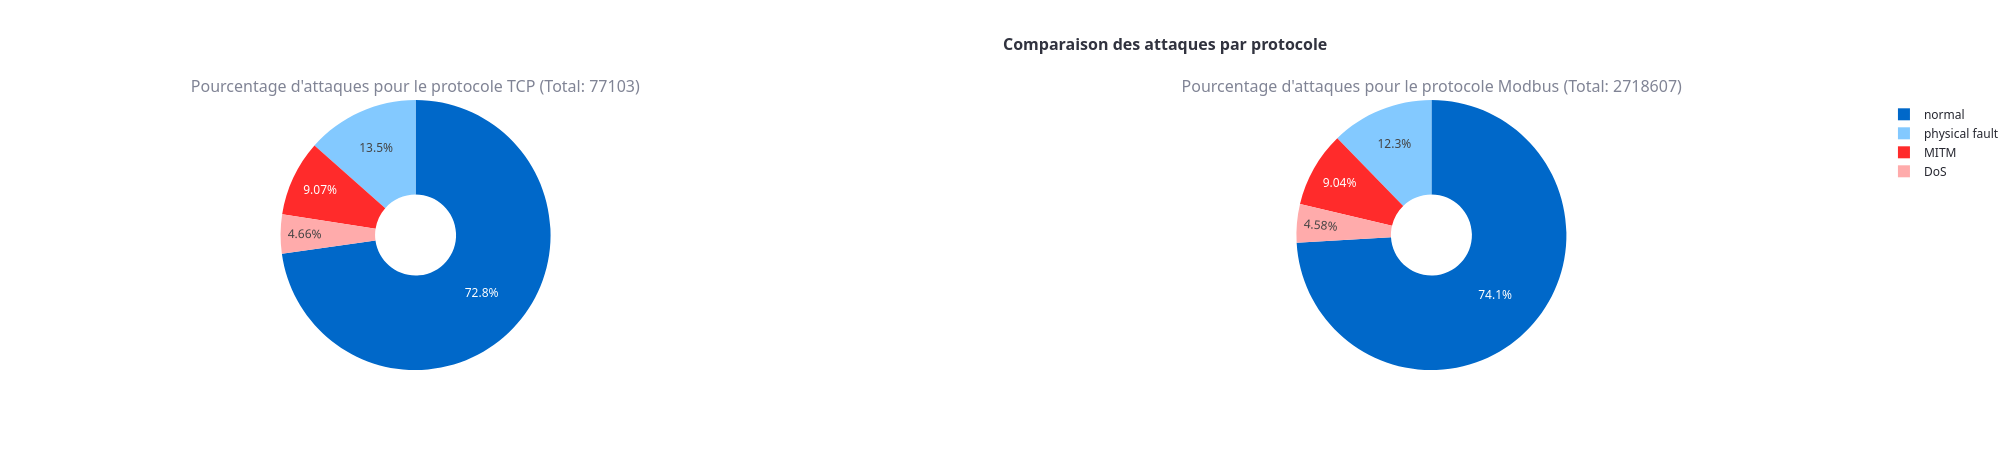
\includegraphics[width=\textwidth]{figures/physical-analysis/attack3.png}
  \vspace{1em} % Espace vertical entre les lignes
  % Deuxième ligne
  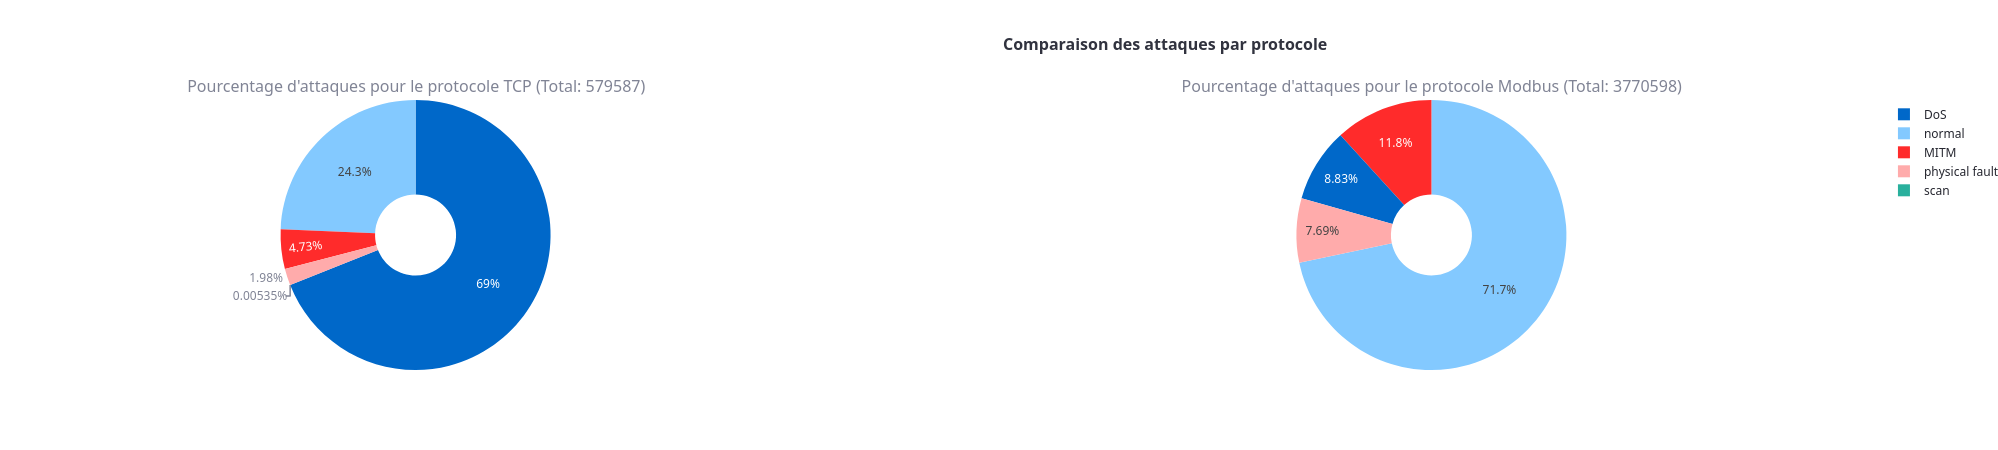
\includegraphics[width=\textwidth]{figures/physical-analysis/attack4.png}
  \caption{Distribution du nombre d'attaques en fonction du nombre de pompes ouvertes}
  \label{fig:network-repartition}
\end{figure}

Les attaques sont réparties de la manière suivante :
\begin{itemize}
  \item La tendance globale montre une majorité de valeurs \texttt{normal} et une minorité de valeurs \texttt{SCAN}.
  \item Pour le protocole TCP, il y a une majorité d'attaques DoS.
  \item Pour le protocole ModBus, il y a une majorité d'attaques MITM.
  \item Pour le DataFrame 1, il n'y a ni d'attaque SCAN ni de DoS.
\end{itemize}

\subsubsection*{Correlation entre les adresses MAC et IP}

\begin{figure}[H]
  \centering
  % Première ligne
  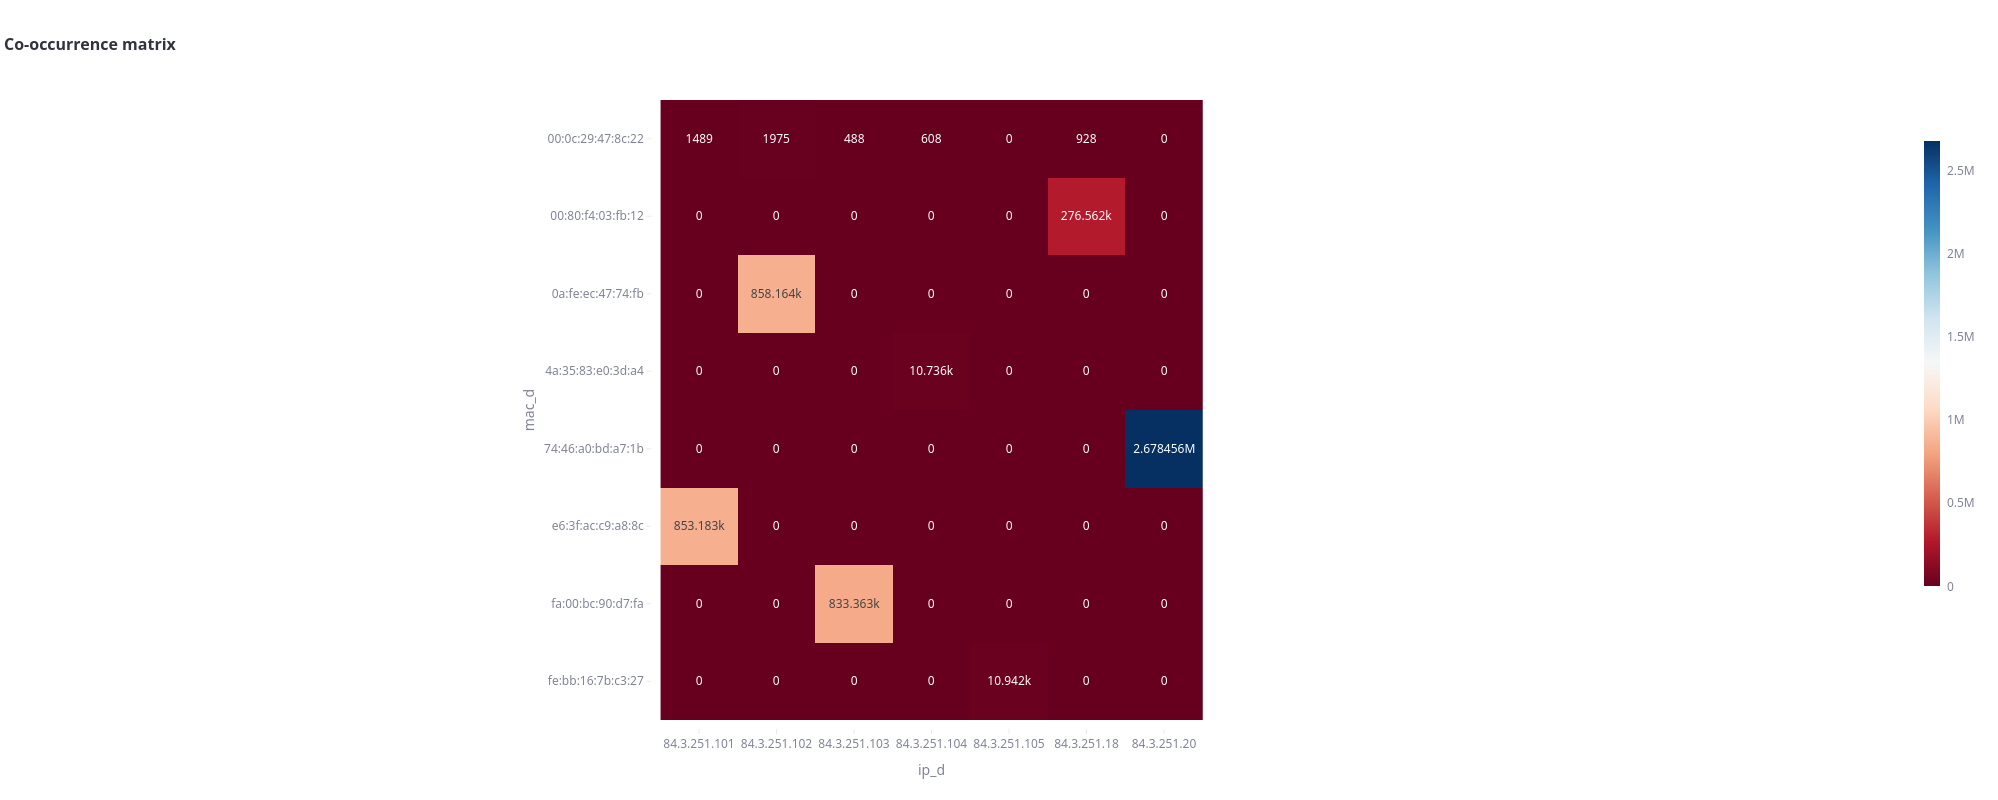
\includegraphics[width=\textwidth]{figures/physical-analysis/co-occurence1.png}
  \caption{Matrice de co-ocurence entre les adresses MAC et IP pour le dataframe 1}
  \label{fig:co-ocurence}
\end{figure}

La figure \ref{fig:co-ocurence} montre que les adresses MAC et IP sont liées : pour une adresse MAC donnée, il y a une adresse IP correspondante. Seule exception, pour le dataset 1, il y a des adresses MAC qui n'ont pas d'IP correspondante.

\subsubsection*{Comparaison des moyennes du nombre de pacquets}

\begin{figure}[H]
  \centering
  % Première ligne
  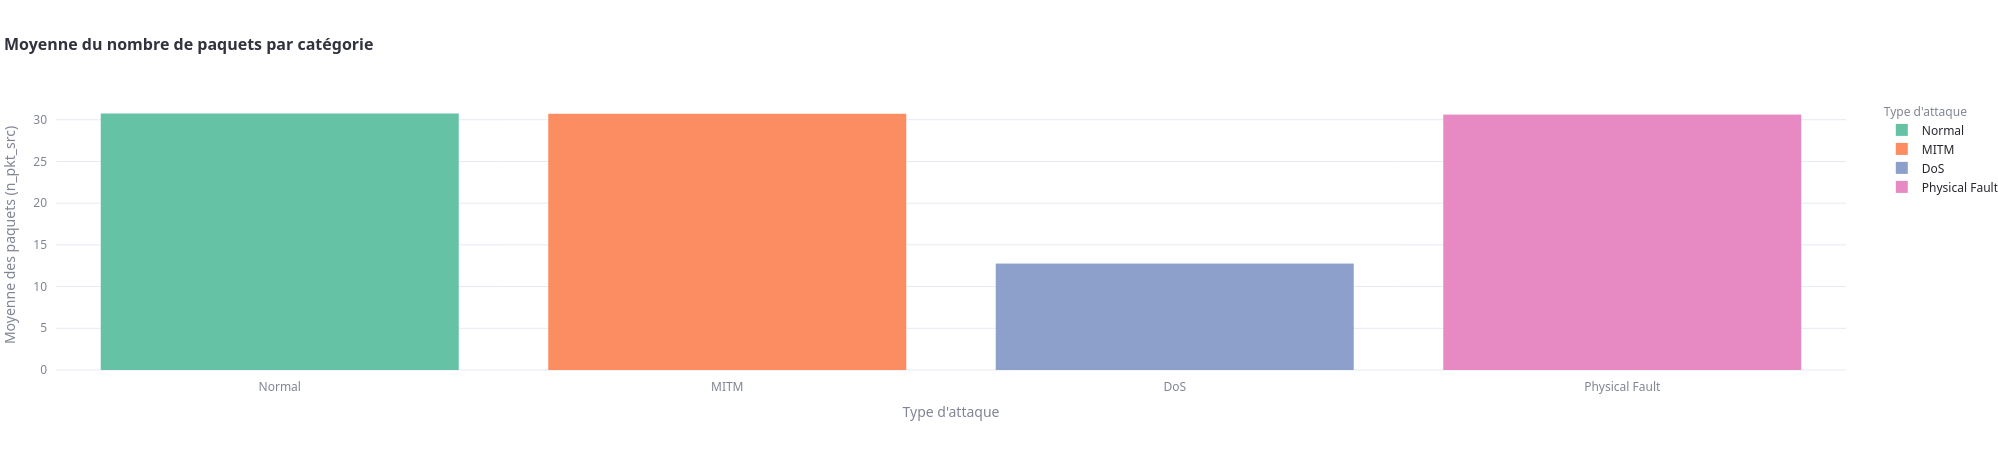
\includegraphics[width=\textwidth]{figures/physical-analysis/mean33.png}
  \vspace{1em} % Espace vertical entre les lignes
  % Deuxième ligne
  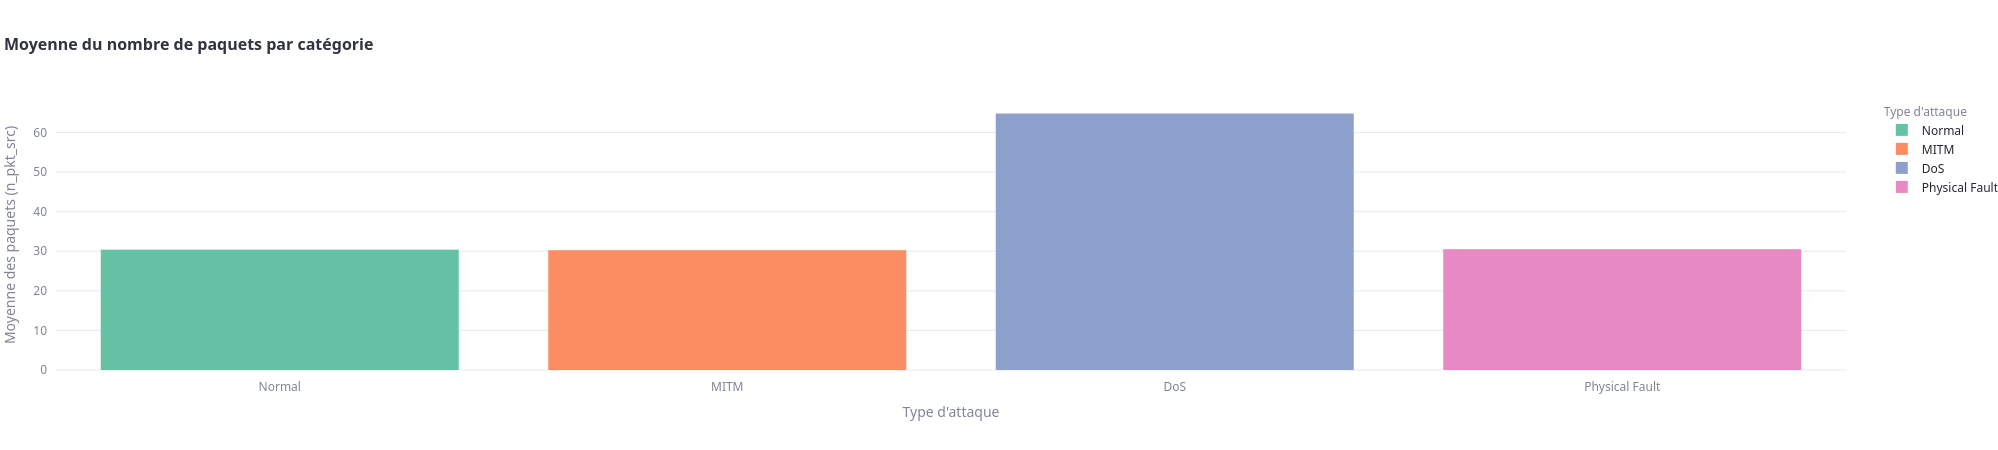
\includegraphics[width=\textwidth]{figures/physical-analysis/mean41.png}
  \caption{Comparaison des moyennes de pacquet pour chaque type d'attaque pour deux dataframes}
  \label{fig:mean}
\end{figure}

La figure \ref{fig:mean} montre que les moyennes sont à des niveaux similaires pour les différents types d'attaques, excepté pour l'attaque DoS. Dans le dataframe 4, il y a plus de pacquets pour les attaques DoS que pour les autres types d'attaques, et dans le 3 il y en a moins.

\subsubsection*{Autres remarques}

Flag discrimine les scans et label\_n permet de détecter les attaques MITM.

